\documentclass[10pt, conference, compsocconf]{IEEEtran}
\usepackage{cite}

% *** GRAPHICS RELATED PACKAGES ***
\ifCLASSINFOpdf
   \usepackage[pdftex]{graphicx}
   \graphicspath{{./images/}}
   \DeclareGraphicsExtensions{.pdf,.jpeg,.png}
\fi

% *** MATH PACKAGES ***
\usepackage[cmex10]{amsmath}

% *** SPECIALIZED LIST PACKAGES ***
\usepackage{algorithm}
\usepackage{algorithmic}

% *** ALIGNMENT PACKAGES ***
\usepackage{array}
\usepackage{mdwmath}
\usepackage{mdwtab}
\usepackage{eqparbox}

% *** SUBFIGURE PACKAGES ***
\usepackage[tight,footnotesize]{subfigure}

% *** FLOAT PACKAGES ***
% \usepackage{fixltx2e}
% \usepackage{stfloats}

% *** PDF, URL AND HYPERLINK PACKAGES ***
\usepackage{url}

\usepackage{color}

% correct bad hyphenation here
\hyphenation{op-tical net-works semi-conduc-tor}

\begin{document}
% use linebreaks \\ within to get better formatting as desired
\title{Scalable Parallel Tracking of Time-Varying 3D Flow Features}

\author {
\IEEEauthorblockN{Authors Name/s per 2nd Affiliation (Author)}
\IEEEauthorblockA{line 1 (of Affiliation): dept. name of organization\\
line 2: name of organization, acronyms acceptable\\
line 3: City, Country\\
line 4: Email: name@xyz.com}
\and
\IEEEauthorblockN{Authors Name/s per 2nd Affiliation (Author)}
\IEEEauthorblockA{line 1 (of Affiliation): dept. name of organization\\
line 2: name of organization, acronyms acceptable\\
line 3: City, Country\\
line 4: Email: name@xyz.com}
}

% make the title area
\maketitle

\begin{abstract}
Large-scale time-varying volume data set can take terabytes to petabytes of storage space to store and process. One promising approach is to process the data in parallel, extract features of interest and analyze only those features, thus reducing required memory space by several orders of magnitude for the following visualization tasks. However, extracting volume features in parallel is a non-trivial task as features might span over multiple processors, and local partial features can be only visible within their own processor. In this paper, we discuss how to generate and maintain connectivity information of features across different processors. Based on this connectivity information, partial features can be integrated, which makes it possible to extract and track feature for large data in parallel. We demonstrate the effectiveness and scalability of our approach using real-world data sets with up to 16384 processors.
\end{abstract}

\begin{IEEEkeywords}
feature tracking; parallel graph;
\end{IEEEkeywords}

\IEEEpeerreviewmaketitle

\section{Introduction}

The accessibility to supercomputers with increasing computing power has enabled scientists to simulate physical phenomena of unprecedented complexity and resolution. These simulations generate large-scale time-varying data that can take tera- or even peta-bytes of space to preserve. Such storage requirement will be not sustainable towards the forthcoming exascale computing. One promising solution to the problem is to reduce the data by storing only features of interest. Extracted features require storage space that can be several orders of magnitude smaller than raw data.

However, it is a non-trivial task to extract and track features embedded in large data. Large simulation data are typically presented and processed in a distributed fashion, simply because of the shear size. A feature can span over multiple distributed data blocks, and its distribution can evolve over time. Existing research effort on feature-based data visualization has mostly focused on extracting features using quantitative measures, such as size, location, shape, and topology information. These methods can extract partial features among individual data blocks, but cannot directly assemble partial features to provide integrated descriptions, unless the distribution of partial features can be captured and traced efficiently over time.

%These measures cannot be applied to distributed volumetric data directly since volumetric features are consist of certain amount of voxels, and are very likely to span over distributed data blocks as they evolve over time. Therefore existing quantitative measures of partial data scattered across different data blocks cannot be used to describe an integrated feature, unless the distribution of partial features can be obtained beforehand.

Efficiently capturing the distribution of features is challenging with respect to increasing numbers of features and computing nodes. In this paper, we present a scalable approach to generating feature residual information and tracking feature connectivity information using parallel machines. Compared to the existing approaches that gather the global feature information in a single host node, our approach only involves local residual data blocks of target features. This requires least communication overhead and avoids the potential link contention. We demonstrate the effectiveness and scalability of our method with real-world vortical flow data sets on large parallel supercomputers with up to 16384.


%To obtain the distribution information of features, a connectivity graph of each feature should be generated and maintained. In this paper, we present an approach to gathering feature residual information and track connectivity information using parallel graphs. Comparing to the existing approaches that generate and maintain the global feature information in a single host node, our approach can be done locally that only involves residual data blocks of target features. This requires least communication overhead and avoids the potential link contention. We demonstrate the effectiveness of this method with \textcolor{red}{two} vortical flow data sets and the scalability of our system in a distributed environment. 
\section{Background and Related Work}

\subsection{Feature Extraction and Tracking}

Feature extraction and tracking are two closely related problems in feature-based visualization. Although many feature tracking algorithms have been introduced, most of them extract features from individual time steps and then try to associate them between consecutive time steps. Silver and Wang \cite{Silver1997} defined threshold connected components as their features, and tracked overlapped features between successive time steps by calculating their differences. Octree was employed in their method to speed up the performance and the criteria they used were domain dependent. Reinders et al.

\cite{Reinders2001} introduced a prediction verification tracking technique that calculates a prediction by linear extrapolation based on the previous feature path, and a candidate will be added to the path if it corresponds to that prediction. Ji and Shen \cite{Ji2003} introduced a method to track local features from time-varying data by using higher-dimensional iso-surfacing. They also used a global optimization correspondence algorithm to improve the robustness of feature tracking \cite{Ji2006}. Caban et al. \cite{Caban2007} estimated a tracking window and then tried to find the best match between that window and different sub-volumes of subsequence frames by comparing their distance of textural properties. Also, Bremer et al. \cite{Bremer2007} described two topological feature tracking methods, one employs Jacobi sets to track critical points while the other uses distance measures on graphs to track channel structures.

Most of the aforementioned methods extract features from each time step independently and then apply correspondence calculations. This could become very slow when the data size becomes large. Muelder and Ma \cite{Muelder2009} proposed a prediction-correction approach that first predicts feature region based on the centroid location of that in previous time steps, and then corrects the predicted region by adjusting the surface boundaries via region growing and shrinking. This approach is appealing because of its computing efficiency and the reliability in an interactive system.

\subsection{Parallel Feature Extraction and Tracking}

To boost the speed for feature tracking in data-distributed applications, Chen and Silver \cite{Chen2003} introduced a two stage partial-merge strategy using master-slave paradigm. The slaves first exchange local connectivity information using Binary-tree merge, and then a visualization host collects and correlates the local information to generate the global connectivity. This approach is not scalable since half of the processors will become idle after each merge. It is also unclear how the visualization host can efficiently collect local connectivity information from non-server processors, since gathering operation is typically very expensive given a large number of processors.

% \textcolor{red}{Shall I compare our work here in the related work section?}
The approach proposed in this paper follows a different strategy. Instead of being sent back to a host, the local connective information is computed and preserved only in the nodes where correspondent features reside. Hence there is no global connectivity information preserved in the host. The host only serves as an interface to broadcast the criterion of feature of interest to the other nodes. In this way, the computation of merging local connectivity information is distributed to the slaves and thus effectively reduces the potential communication bottleneck on the host.

Moreover, our approach does not need a global synchronization for gathering all local connectivity information at the host, hence avoids potentially long computation time caused by features spanning over a large number of nodes. In addition, there are no needs to set a barrier to wait for all connectivity information being sent back to the host and thus if there exists features that span over a large number of nodes but was not selected by the user, the potentially long computation time for these features will not block the whole process. This makes it ideal for an interactive system, where users can select the features of interest and instantly receive the visual feedback as the features evolves.

\subsection{Parallel Graph Algorithm and Applications}

Graph-based algorithms have long been studied and used for a wide range of applications, typically along the line of divide-and-conquer approaches.
Grundmann et al. \cite{Grundmann2010} recently proposed a hierarchical graph-based approach for video segmentation, a closely related research topic to 3D flow feature extraction as video can be treated as a space-time volume of image data \cite{Klein2002}. In their work, a connected sequence of time-axis-aligned subsets of cubic image volumes are assigned to a set of corresponding processors, and incident regions are merged if they are inside the volumes window. Incident regions on window boundary, however, are first marked as ambiguous and later connected by merging neighboring window to a larger window, which consists of the unresolved regions form both window on their common boundary. This approach is not applicable for memory intensive situation since the allocated volume size before merging might already reaches the capacity. Same restriction applies to the parallelized BK algorithm \cite{Boykov2004} proposed by Liu and Sun \cite{Liu2010}, in which data are uniformly partitioned and then adaptively merged to achieve fast graph-cuts. These approaches are suitable for shared-memory but not message-passing parallelization as for their frequent shifting on data ranges.
% \textcolor{red}{Not enough, need to read more.}
\section{Overview}

It is challenging to extract and track features of large time-varying volume data in parallel. First, although a feature can be extracted partially on a processor using the conventional methods, we need to build the connectivity information of the feature across multiple processors. Such information allows us to obtain the global description of a feature from a set of neighboring processors, and enables more advance operations such as similarity evaluation. Second, such connectivity information can be dynamically changed with feature evolving over time. We need to update and maintain the connectivity of features in an efficient fashion to track highly intermittent phenomena.

%The biggest challenge for tracking large time-varying volumetric data set lies in that, though features can be extracted within individual processors using the conventional methods, they might also span over multiple data blocks, which is unavoidable as the number of processors increases. To extract and trace a feature over a distributed volume data set, we need to build and maintain the connectivity information of the features across multiple nodes. As feature descriptors, such as size, curvature, and velocity, are distributed among processors, connectivity information can facilitate us to obtain the description of a feature from neighboring processors, and also enable more advanced operations such as similarity evaluation.

However, it typically requires intensive data exchanges among processors to build and maintain connectivity information of features, and thus incurs extra communication cost. To address this issue, we adopt the master-slave paradigm~\cite{Chen03realtime}, but design a different strategy. Instead of being sent back to a host, the local connective information is computed and preserved only in the slaves where the correspondent features reside. Hence there is no global connectivity information preserved in the host. The host only serves as an interface to broadcast the criterion of features to the slaves. In this way, the computation of merging local connectivity information is distributed to the slaves. Thus, we can effectively reduce the potential communication bottleneck on the host.

In addition, our approach does not need a global synchronization for gathering all local connectivity information at the host, thus avoiding potentially long computation time caused by features spanning over a large number of nodes. Furthermore, there are no needs to set a barrier to wait for all connectivity information being sent back to the host. Thus, if there exists features that span over a large number of nodes but are not explored by the user, the potentially long computation time for these features will not block the whole process. This makes it ideal for an interactive system, where users can select the features of interest and instantly receive the visual feedback as the features evolves.

%Our implementation uses a similar system structurer that forms the basis of previous work \cite{Muelder2009}. Figure~\ref{fig:system-overview} depicts a high-level overview of the work flow for a single time-step.
%
%\begin{figure}[ht]
%	\centering
%	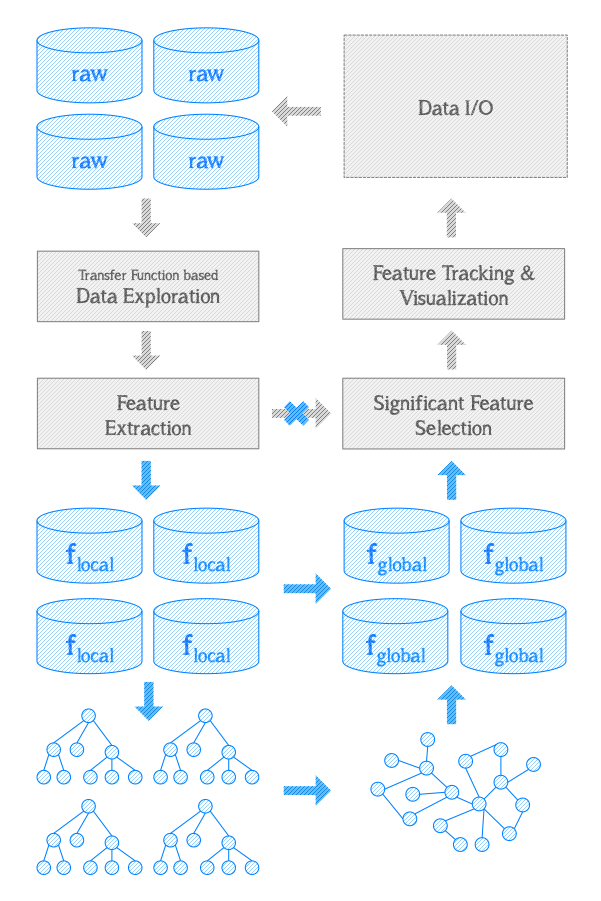
\includegraphics[width=1\linewidth]{system_overview.png}
%	\caption{Work flow of a single time-step}
%	\label{fig:system-overview}
%\end{figure}
%
%First, the source volume data is read either from a pre-generated data set or from a simulation program in-situ. Then, user can identify features of interest via transfer function manipulation as such candidate features will be extracted. However, since the descriptive power of a transfer function is often insufficient to precisely highlight the desired subset of features, user may have to select significant features either by simple point-and-select or iteratively filter out unwanted ones using different feature descriptors. Once the user has identified the interesting features, the system tracks only these significant features in subsequent time steps.
%
%What our approach distinct from that of the previous one lies in that the global connectivity information of each feature need to be obtained before the Significant Feature Selection process could be carried out. As shown in blue color in Figure~\ref{fig:system-overview}, first the raw data are distributed in \textcolor{red}{logically adjacent data blocks.}. After Feature Extraction is done in each data block, the set of local features as well as the local connectivity information will be generated. Then by applying our merging algorithms, global connectivity information can be obtained efficiently such that each data block will possess the global connectivity information for each of its residing features. This enables Signification Feature Selection in a distributed environment and henceforth Feature Tracking and Visualization. 
\section{Methodology}
The biggest challenge for tracking large time-varying volumetric data set lies in that, though features can be extracted within individual processors using the conventional methods, they might also span over multiple data blocks, which is unavoidable as the number of processors increases. To extract and trace a feature over a distributed volume data set, we need to build and maintain the connectivity information of the features across multiple nodes. As feature descriptors, such as size, curvature, and velocity, are distributed among processors, connectivity information can facilitate us to obtain the description of a feature from neighboring processors, and also enable more advanced operations such as similarity evaluation.

However, it typically requires data exchanges among processors to build and maintain such connectivity information, and thus incurs extra communication cost. To design a proper communication scheme for better performance and scalability, we carefully consider the following three factors in our design:

\begin{itemize}
	\item $N_{com}$ : The amount of communication required to build the connectivity graph;
	\item $N_{proc/com}$ : The number of processors involved in each communication;
	\item $N_{data/com}$ : The amount of data that must be changed in each communication.
\end{itemize}

In the following sections, we give a detailed description on how to create and maintain such connectivity information using tree structures and then merge them into an undirected unweighted graph to minimize the cost over the above three factors.

\subsection{Feature Extraction}

In general, a feature can be any interesting object, structure or pattern that is considered relevant for investigation. Here, a feature is defined as the collection of voxices encompassed by a certain iso-surface. Such volumetric feature could be extracted by conventional techniques such as region growing, geometry or topology based clustering, or other domain specific algorithms. In our work we use a standard region-growing algorithm
%\textcolor{red}{why?} %
\cite{Huang2003} to partition the original volume data into an initial set of features. This can be done by first spreading a set of seeding points inside the volume, and then clustering voxices into separate regions, each regarded as a single feature. After specific features have been identified from a single time step, we can track their evolution over time using a prediction-correction approach \cite{Muelder2009}, as feature locations should be consistent for consecutive time step provided that the sampling interval is sufficiently small. Once the prediction is made, the actual region can be obtained by adjusting the surface of the predicted region: first shrink the edge surface points to obtain the mutual region between consecutive time steps, and then use of a region-growing method to generate the refined region, as depicted in Figure~\ref{fig:predict-correct}. This prediction-correction approach was proved effective and efficient for tracking feature on a single processor \cite{Muelder2009}. However, when the size of the volume becomes too large to be able to fit into a single processor, a cluster of processors is often needed so as to process the data in parallel.

%------------------------------------------------
\begin{figure}[ht]
	\centering
	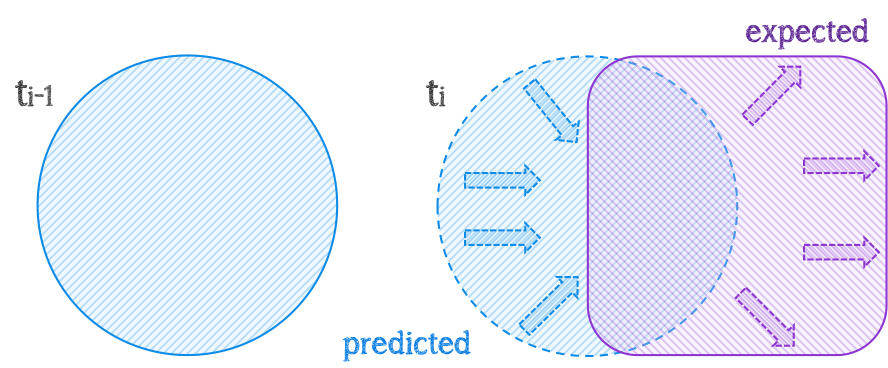
\includegraphics[width=0.9\linewidth]{predict_correct.png}
	\caption{The predict-correct feature tracking approach. First the predicted region is derived using location(s) of that feature in previous time step $t_{i-1}$. Then we shrink the portion that does not satisfy the criteria in $t_i$, which obtain us the mutual portion of that in $t_{i-1}$ and $t_i$. Finally we apply region growing again to obtain the expected feature region depicted.}
	\label{fig:predict-correct}
\end{figure}
%------------------------------------------------

One challenge to parallelize the tracking approach lies in that it can be difficult to obtain the global feature descriptions unless they can be shared and merged in an efficient way. This is because the features may span over multiple processors and partial features in different data blocks are operated independently. An intuitive way of exchanging such feature information is to first find how features span over multiple processors, and then merge them according to the connectivity information.

\subsection{Creating Local Connectivity Tree}

If we partition a volumetric data set into a regular grid of data blocks, it is very likely that some of the features will cross multiple blocks. Leveraging that the cross-section of such feature in both side of adjacent blocks should match, we could connect separate parts of a feature in adjacent blocks by comparing their cross-sections on correspondent boundary surfaces.

Since data is distributed, each processor is not aware of the partial features identified on the other processors. Though exchanging the voxels on the sectional area between two adjacent processors would be sufficient for finding possible matches of partial features, we choose to exchange more abstract data to find matches:

\begin{itemize}
	\item $P_{centroid}$: The geometric centroid of the cross-sectional area.
	\item $P_{min-max}$: The minimal and maximal (min-max) coordinate of the cross-sectional area;
\end{itemize}

The reason why we choose geometric centroid instead of introducing a voxel-width "ghost surface" is that it requires much less communication cost. A ghost surface that stores boundary surface belonging to neighboring blocks might help to achieve voxel-wise matching for partial features. However, maintaining such ghost surfaces requires frequent inter-process communication and is considerably expensive for data generated in real-time. Consider the fact that it is rarely the case that a feature will have a sharp \textcolor{red}{half-dome-like} sectional plane right on the boundary surface, we can loose the matching criterion by allowing a 1-voxel offset between two correspondent geometric centroids. Together with the min-max coordinate of the cross-sectional area, bipartite matching of partial features could be achieved, as shown in Algorithm~\ref{alg:match}.

%------------------------------------------------
\begin{algorithm}
\caption{Match of two partial features}
	\begin{algorithmic}
		\IF{$P_{centroid}$ = $P_{centroid}^{'}$ \textbf{and} $P_{min-max}$ = $P_{min-max}^{'}$}
			\STATE return $f$ \textbf{matches} $f^{'}$
		\ENDIF
	\end{algorithmic}
\label{alg:match}
\end{algorithm}
%------------------------------------------------

Another reason the min-max coordinate values are not optional is because they ensure correct connectivity for some special cases where one cross-sectional area is surrounded by another concave or hollow area whose centroid points happen to be the same, as depicted in Figure~\ref{fig:special}.

%------------------------------------------------
\begin{figure}[ht]
	\centering
	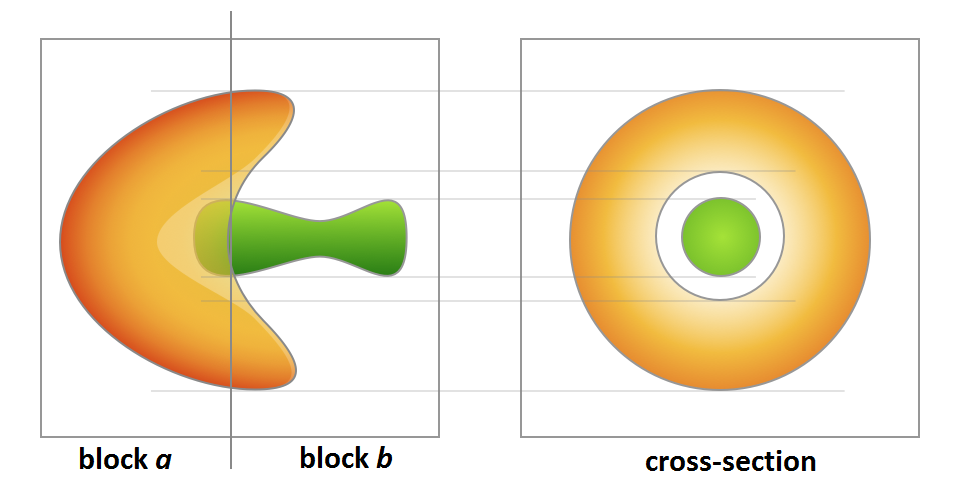
\includegraphics[width=0.9\linewidth]{figure1@2x.png}
	\caption{A special case where two features share the same centroid on the section.}
	\label{fig:special}
\end{figure}
%------------------------------------------------

Based on the afore-explained fact that partial features could be connected by finding matches, we can abstract the local connectivity information using a tree structure as depicted in Figure~\ref{fig:match}. For each data block in the grid, there will be six direct neighbors (the outermost blocks have less), each with a sharing boundary surface with the current block. The connectivity tree is constructed taking the current block as root, its six adjacent blocks as its first level child nodes, and a new leaf is appended to each surface node if a local feature touches the block boundary surface.

%------------------------------------------------
\begin{figure}[ht]
	\centering
	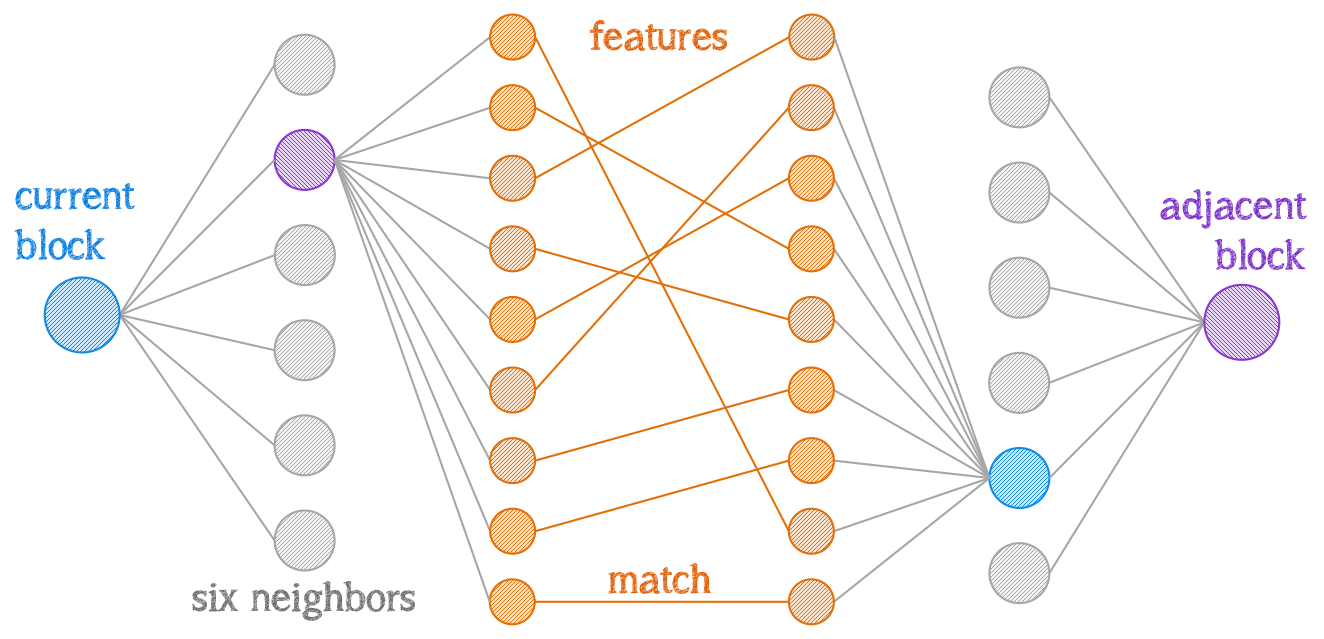
\includegraphics[width=1\linewidth]{match.png}
	\caption{The tree structure used for maintaining local connectivity information, where the root node is encoded with the current block index, its child nodes the index of its neighboring blocks, and for each child node its leaves represent local on-boundary-features. The leaves should match that reside in the corespondent neighboring block, leveraging which a connectivity graph can be constructed.}
	\label{fig:match}
\end{figure}
%------------------------------------------------

Note that each voxel in the local data block has a unique global index, each leaf could thus be encoded using 3 integers (global index for $P_{centroid}$, $P_{min}$ and $P_{max}$), we use the index of $P_{centroid}$ as the feature index, and sort the sibling leaves according to its index in ascending order. On the other hand, the root and the first level child nodes can be encoded with the index of corresponding data blocks, which is irrelevant to the number of feature-on-boundary (henceforth referred as $N_{fb}$). Therefore the overall spatial complexity of creating local connectivity tree for each data block is ($\theta(3*N_{fb})$). \textcolor{red}{Consider an extreme case that there are 10k features touching each side of the boundary surface, the total memory needed for the local connectivity tree is only $((3*10000 + 1)*6 + 1) * 4 bytes \approx 720KB$, neglectable comparing to the volume size itself.}

From the temporal complexity perspective of view, the creation of local connectivity tree will not introduce extra computational cost as it can be done along with the region growing process. The value of $P_{centroid}$ and $P_{min-max}$ are updated only if the feature reaches the boundary surface, hence the temporal complexity for creating the local connectivity tree remains ${O(\sqrt[2/3]{N_{vexol}})}$, a magnitude less than \textcolor{red}{$O(extraction)$.}

Algorithm~\ref{alg:local} shows the detailed algorithm of creating local connectivity tree in the region growing process.
%------------------------------------------------
\begin{algorithm}
\caption{Creating Local Connectivity Tree}
\label{alg:local}

\begin{algorithmic}
	\IF{$t = t_0$}
		\STATE $seeds \leftarrow randomVortices()$
		\FOR {each $seed$ in $seeds$}
			\STATE $feature \leftarrow expendRegion()$
			\STATE append $feature$ to $featureList$
		\ENDFOR	
	\ELSE
		\FOR {each $feature$ in $featureList$}
			\STATE $feature \leftarrow predictRegion()$
			\STATE $feature,P_{centroid},P_{min-max} \leftarrow \textbf{adjustRegion()}$
			
			\STATE $leaf \leftarrow LEAF(P_{centroid}, P_{min-max})$
			\STATE append $leaf$ to $connectivityTree$
		\ENDFOR
	\ENDIF
\end{algorithmic}

\begin{algorithmic} \STATE \end{algorithmic}	% line separator

\begin{algorithmic}
\STATE $\textbf{adjustRegion:}$
	\IF{Voxel $v$ on boundary surface}
		\STATE $P_{centroid} \leftarrow updateBoundaryCentroid()$
		\STATE $P_{min-max} \leftarrow updateMinMaxBoundary()$
	\ENDIF
\end{algorithmic}
\end{algorithm}
%------------------------------------------------

\subsection{Creating Global Connectivity Graph}

After local connectivity trees have been created within each data block, their leaves need to be exchanged and merged to obtain the overall description of a partitioned feature. The exchanging and merging process is decisive that their effectiveness will largely affect the overall performance and scalability of the feature tracking algorithm as a whole.

In this subsection, we start with a naive solution and discuss progressively through different data exchanging strategy for different scenarios.

\subsubsection{The Naive Solution}

A naive solution to obtaining global connectivity information for each feature-on-boundary is to exchange its corresponding leaf with its targeting block. Recall that the first level child nodes are encoded as the ranks of adjacent blocks, and the leaves the global index of the geometric centroid and the min-max boundary on the shared boundary surface. Therefore if a leaf received from neighboring data block matches a local leaf, the two leaves, that is, the two partial features they represented, must share the same boundary section with the same centroid and section region. In other word, these two partial features are resulted by partitioning a original feature, and should be considered as the same feature.

To prevent a leaf from being resending to the same neighboring block multiple times, it is marked as sent and unless the same feature was found partially reside in another neighboring block, this leaf will be ignored in the next communication to reduce $N_{data/com}$.

Algorithm~\ref{alg:merge} shows the detailed process to merge matched leaves.
%------------------------------------------------
\begin{algorithm}
\caption{Merging Matched Leaves}
\label{alg:merge}
\begin{algorithmic}
\STATE traverse local connectivity tree in preorder
\FOR {each $f_{local}$ in $localLeaves$}
	\IF{$f_{local}$ is sent = false}
		\STATE send $f_{local}$ to targeting block
	\ENDIF
	\STATE mark $f_{local}$ as sent
\ENDFOR
\FOR {each $f_{recv}$ in $recievedLeaves$}
	\FOR {each $f_{local}$ in $localLeaves$}
		\IF{$f_{recv}$ \textbf{matches} $f_{local}$}
			\STATE $f_{local}.id = min(f_{recv}.id, f_{local}.id)$
			\STATE mark $f_{local}$ as not sent
		\ENDIF
	\ENDFOR	
\ENDFOR
\end{algorithmic}
\end{algorithm}
%------------------------------------------------

The naive solution may work for data sets with feature-on-boundary that span only a few number of blocks. However, if there exists long curly features partitioned evenly over the data block grid, each block needs to consecutively communicate with its neighbors to incrementally gather and merge a global feature. This requires O(${N_p}$) communications to connect a single feature, where ${N_p}$ is the number of processors in the grid. Consequently, the total communication cost is O(${N_{fb} \times N_p}$) times communication. In addition, since one processor cannot predict how many leaves it will receive from its adjacent processors, it is hard to schedule the communication process.

%------------------------------------------------
% \begin{figure*}[ht]
%   \centering
%     \subfigure[Local connectivity tree]{
%       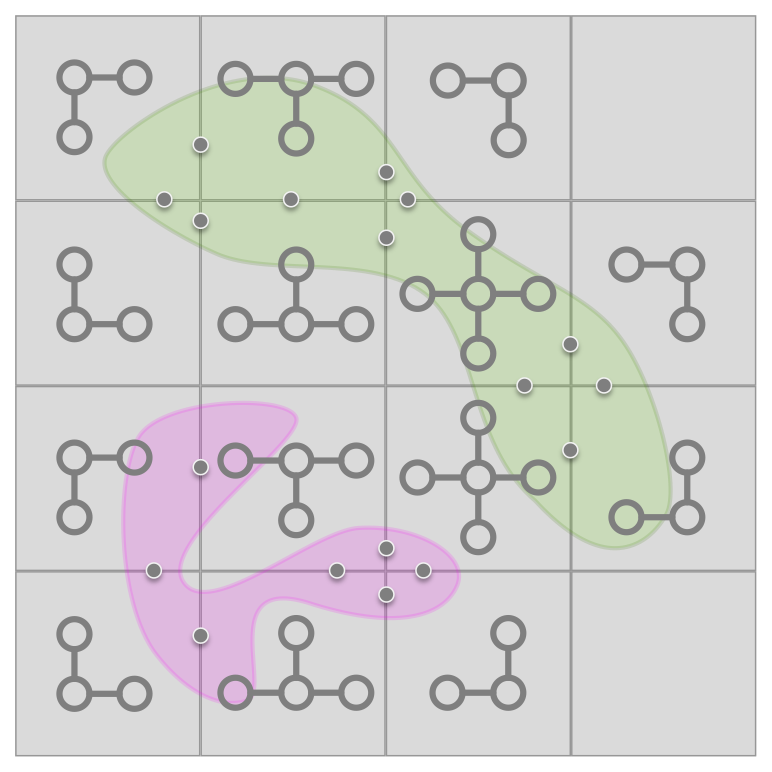
\includegraphics[width=0.23\linewidth]{create.png}
%       \label{fig:create}
%     }
%     \subfigure[Centralized merge with host]{
%       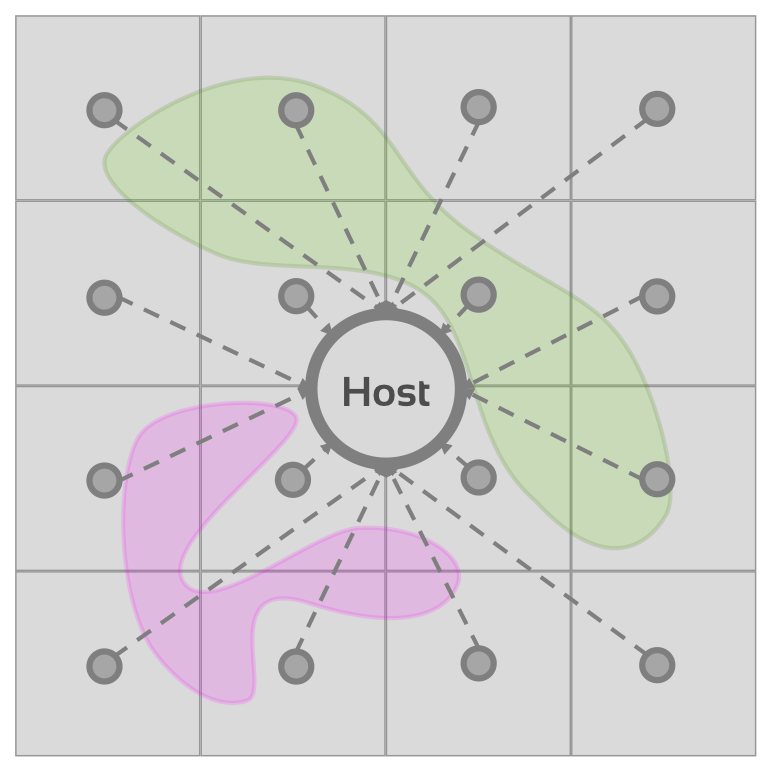
\includegraphics[width=0.23\linewidth]{host.png}
%       \label{fig:host}
%     }
%     \subfigure[Centralized merge without host]{
%       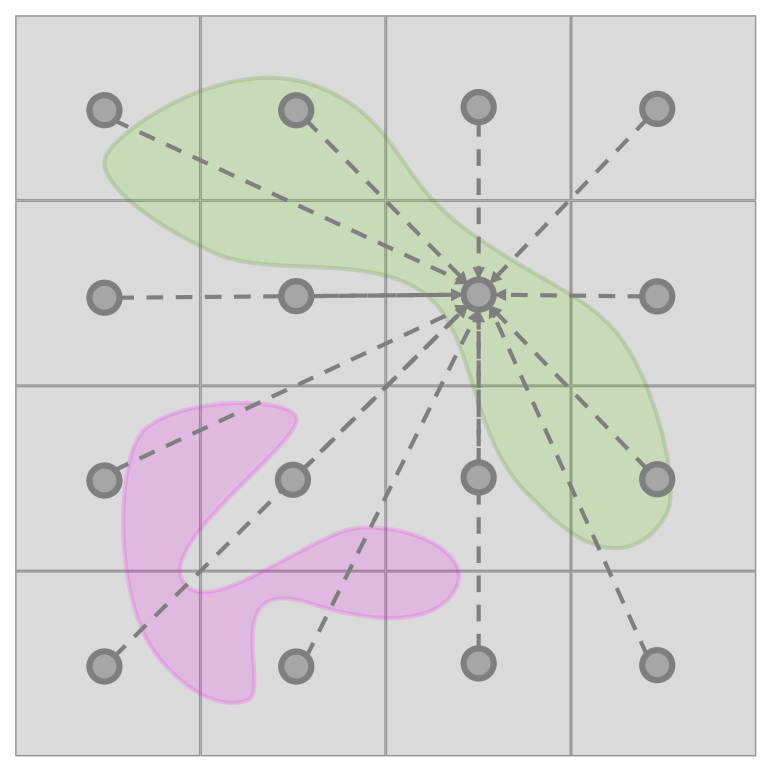
\includegraphics[width=0.23\linewidth]{centralized.png}
%       \label{fig:centralized}
%     }
%     \subfigure[Decentralized merge]{
%       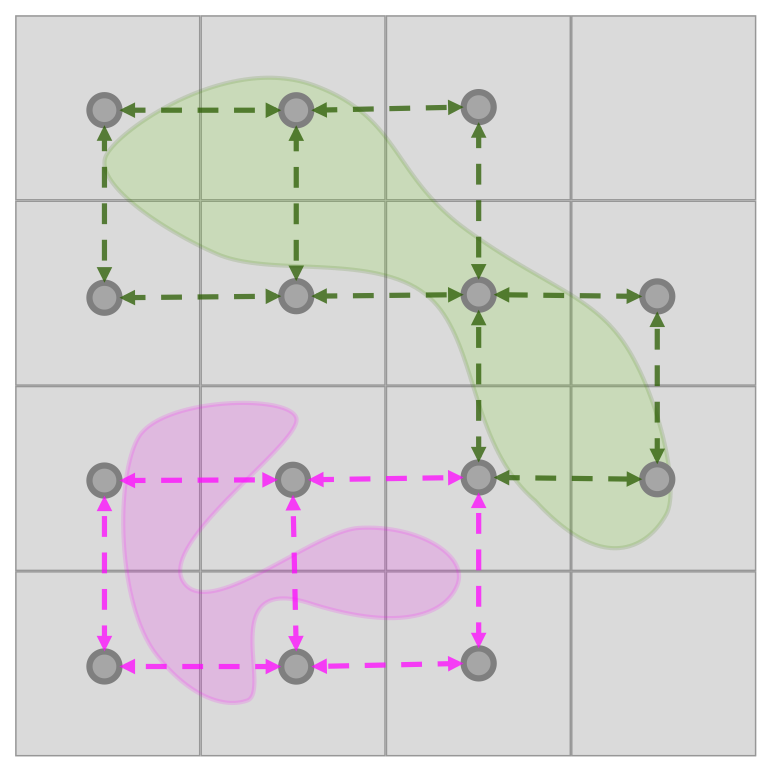
\includegraphics[width=0.23\linewidth]{decentralized.png}
%       \label{fig:decentralized}
%     }
%   \caption[Optional caption for list of figures]{Caption of subfigures \subref{fig:create}, \subref{fig:centralized} and \subref{fig:decentralized}}
% \end{figure*}
%------------------------------------------------

\subsubsection{The Centralized Approach}

One possible solution to improve the aforementioned \textcolor{red}{serialized} approach is to introduce master-slave hierarchy to reduce the number of communication required for merging all leaves. The master-slave hierarchy can be constructed using a separate host processor. When the feature extraction process is done, all local connectivity trees are gathered to the host processor. Then the host nodes starts to merge the leaves from each connectivity tree to construct a single global connectivity graph.

The merit of this centralized approach lies in that it requires inter-processor communication only once, ($N_{com} = 1$). Moreover, the global graph of feature information can be preserved in the host that it can response to feature queries directly without collecting information from the slaves again. However, this approach has an obvious drawback. Since all local connectivity trees are sent to the host, the number of processors involved in each communication is $N_{proc/com} = N_p$, and there exists potential bottlenecks, both in communication and computation, on the host.

\subsubsection{The Decentralized Approach}

A better solution is to decentralize the gathering and merging process from a single host processor to all processors available. After the feature extraction process is done and so does the creation of local connectivity tree, an \emph{all-gather} process starts to exchange all local connectivity trees within each data block to all the others. Each block will first collect a full copy of all local connectivity trees followed by the same process as mentioned in Algorithm~\ref{alg:merge} to merge the leaves into a single concise connectivity graph.

Though the "redundant" host processor is no longer required when applying for computation resources, this approach does not actually resolve the bottleneck problem since now every processor is acting like the host for that they still need to gather all local trees and to merge them \textcolor{red}{simultaneously}. For real world data set however, it is rarely the case that all features will span over every data block. In other word, it is unnecessary for one processor to gather leaves of features that are not local. To reduce the redundant communications with every other data block in the grid, the decentralized approach could be further improved to communicate with only those data blocks that are directly adjacent. That is, each data block only communicates with its direct neighbors and shares information with them regardless what is happening outside.

For a regularly partitioned volumetric data set, there are at most six direct neighbors for each data block. Instead of gathering connectivity information from all non-current data blocks in the grid, we let each data block gather only new leaves from its neighboring blocks within each communication. This could be considered as a higher level of region growing process, starts from one seeding block and grows to adjacent blocks by exchanging and merging connectivity information in a bread-first fashion, until all cross-boundary features are connected. Figure~\ref{fig:grid2d} gives an example of the process of processor-level region growing in a 2D processor grid.

%------------------------------------------------
\begin{figure}[ht]
	\centering
	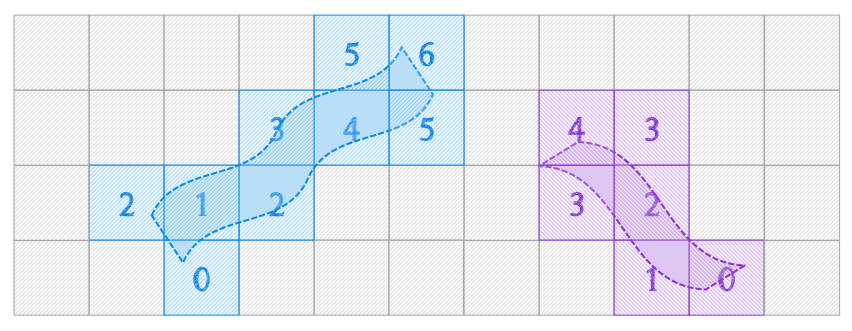
\includegraphics[width=1\linewidth]{grid2d.png}
	\caption{The processor-level region growing process in a 2D grid, in which it takes a maximum of 2n-1 times (3n-1 for 3D grid) for the outermost processor to grow to the furthest processor}
	\label{fig:grid2d}
\end{figure}
%------------------------------------------------

The reason we choose the six-direct-neighbor paradigm is because it gives the minimum overall computational complexity. It takes a maximum of ${3n-1}$ times communication, where \emph{n} denotes the longest side length, for any data block to receive connectivity information from the furthest block on the opposite diagonal. The temporal complexity for garnering all necessary leaves is hence as low as ${O(\sqrt[3]{N_{proc}})}$. And the number of processors involved in each communication is a constant of a maximum of six ($N_{proc/com} \leq 6$).

Another optional paradigm is to let each processor communicate with its 26 neighbors, including the adjacent diagonal blocks. Communicate with the adjacent diagonal block takes as much as half the time for any block to reach its furthest diagonal. However, $N_{proc/com}$  is also increased to 26. For data sets that features span over all blocks are subordinate, six-direct-neighbor paradigm outweighs the 26-neighbors paradigm in computational complexity.

To schedule the communication with neighboring blocks, we use two schedule flags, \emph{toSend} and \emph{toRecv}, to indicate whether a block need to send or receive leaves to/from its neighboring blocks. Whenever a block receives leaves that can be merged into its existing connectivity graph, we assume the neighboring blocks might receive further connectivity information from their neighbors. In this case, the \emph{toRecv} flag is set to true until the connectivity graph is \textcolor{red}{saturated}; On the other hand, the \emph{toSend} flag is set in accordance to whether one of the neighboring blocks need to receive leaves, which can be obtained by gathering the neighboring \emph{toRecv} flags. Each data block will keep exchanging connectivity information until both \emph{toSend} and \emph{toRecv} flags are set to false.

The detailed scheduling algorithm is depicted in Algorithm~\ref{alg:schedule}.
%------------------------------------------------
\begin{algorithm}
\caption{Decentralized Local Merge}
\label{alg:schedule}
	\begin{algorithmic}
	\STATE $toSend, toRecv \leftarrow true$
	\STATE $\delta \leftarrow localLeaves$
	\WHILE {$toSend$ is true \textbf{or} $toRecv$ is true}
		\STATE $target \leftarrow myRank$ \textbf{if} $toRecv$ = $true$
		\STATE $procsToSync \leftarrow gatherNeighbor(target)$
		
		\FOR {each $proc$ in $procsToSync$}
			\IF {$toSend$ = $true$}
				\STATE send $\delta$ to $proc$
			\ENDIF
			\IF {$toRecv$ = $true$}
				\STATE receive $\delta\prime$ from $proc$
			\ENDIF
		\ENDFOR
		
		\STATE $toSend \leftarrow false$ \textbf{if} $procsToSync$ is empty \textbf{else} $true$
		\STATE $toRecv \leftarrow false$ \textbf{if} $\delta$ = $Merge(\delta, \delta\prime)$ \textbf{else} $true$
		\STATE $\delta \leftarrow Merge(\delta, \delta\prime)$ \textbf{if} $toRecv$ is true
  \ENDWHILE
  \end{algorithmic}
\end{algorithm}
%------------------------------------------------

\subsubsection{The hybrid approach}

Consider the fact that as data evolves over time, the volumetric features may drift but should not change drastically in neither size, shape nor location if the sampling interval when generating the data is sufficiently small. Base on this assumption, we can further optimizing the aforementioned decentralized-local-merge approach. Utilizing the prediction-correction approach for single processor feature tracking we can further reduces the communication cost required to complete the whole connectivity graph.

\begin{figure}[ht]
	\centering
	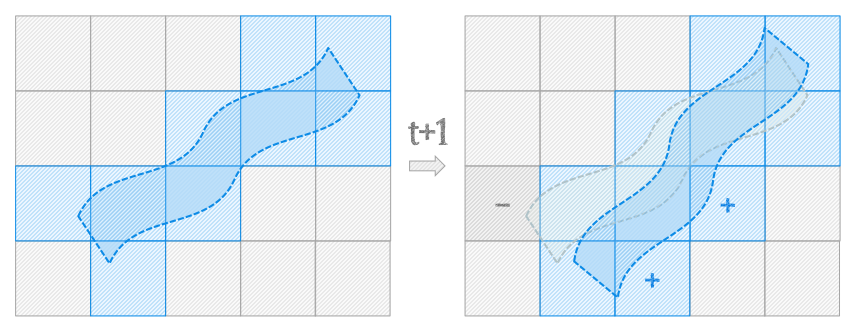
\includegraphics[width=1\linewidth]{hybrid.png}
	\caption{Utilizing the prediction-correction for fast connectivity information synchronization. In each time step the }
	\label{fig:hybrid}
\end{figure}

As depicted in as depicted in Figure~\ref{fig:hybrid}, for every time step $t_i$, when the global connectivity graph is obtained, the local communicators will be updated for the next time step, $t_{i+1}$, with the union of processors that share the same set of feature-on-boundary with the current processor. The leaves from these data blocks are necessary to complete the global connectivity graph no matter which gathering approach is used. Hence, for these must-involve data blocks, we apply the all-gather-decentralize approach, allowing the minimum one-time synchronization to finish gathering all leaves that are necessary for updating the connectivity graph based on the graph created at the previous time step $t$. Then, processor-level region growing, a.k.a the processor-level-decentralize approach is applied to extend the boundary of data blocks, obtaining newly connected blocks caused by the evolution of the volume data. Again, only those leaves that are changed and not yet sent will be exchanged. This ensure that we minimize the amount of data being sent over network.

The detail algorithm of the hybrid approach is given in Algorithm~\ref{alg:hybrid}.
%------------------------------------------------
\begin{algorithm}
\caption{Prediction-enabled Local Merge}
\label{alg:hybrid}
	\begin{algorithmic}
		\STATE Let $P_{f_i} \equiv$ all processors that contains feature $f_i$
		\IF{$t = t_0$}
			\STATE $localCom \leftarrow union(P_{f_i})$ for all $f_i$ in current data block
		\ELSE
			\FOR {each $proc$ on boundary of $localCom$ \textbf{do}}
				\STATE $P_{f_i}^{'} \leftarrow decentralizedLocalMerge(proc)$
			\ENDFOR
			\STATE $localCom \leftarrow union(P_{f_i}^{'})$
		\ENDIF
	\end{algorithmic}
\end{algorithm}
%------------------------------------------------
%-------------------------------------------------------------------------
\begin{figure}[t]
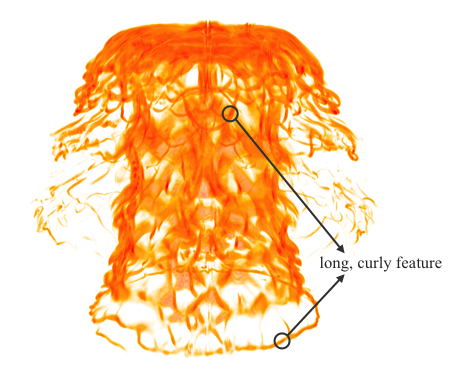
\includegraphics[width=0.9\linewidth]{combustion_labeled.png}
\caption{The volume rendering of a single time step of the combustion data set.}
\label{fig:combustion-labeled}
\end{figure}
%-------------------------------------------------------------------------

\section{Results}

We first test our feature extraction and tracking algorithm on a $256\times256\times256$ vortex data set obtained from a combustion solver that can simulate turbulent flames. In this data set, each voxel contains the magnitude value of vorticity derived from velocity using a curl operator. As time evolves, vortical features may vary from small amassed blob features to long curly features that span over large portion of the volume, as shown in Figure~\ref{fig:combustion-labeled}.

%\subsection{Performance Result}

The volume data can be generated either in advance or on the fly, and thus we ignore the I/O cost and only focus on the computation time for the following three portions.

\textbf{Time for extracting features ($T_{extract}$).}
%
Since we use the region-growing based algorithm to extract features, given a fix specification of features, the computation time is mainly determined by the size of the volume as well as the number of processors being used. Once the raw volume data and its partitioning, a.k.a. the size of each data block is determined, the computation time for extracting residing features remains approximately the same. In post-processing, the size of each data block decreases with the increasing number, and hence so does the time spent on extracting features. As depicted in Figure~\ref{fig:feature-extraction}, $T_{extract}$ is approximately log-linear decreased as the number of processors grows from 8 to 16384.

\begin{figure}[t]
\centering
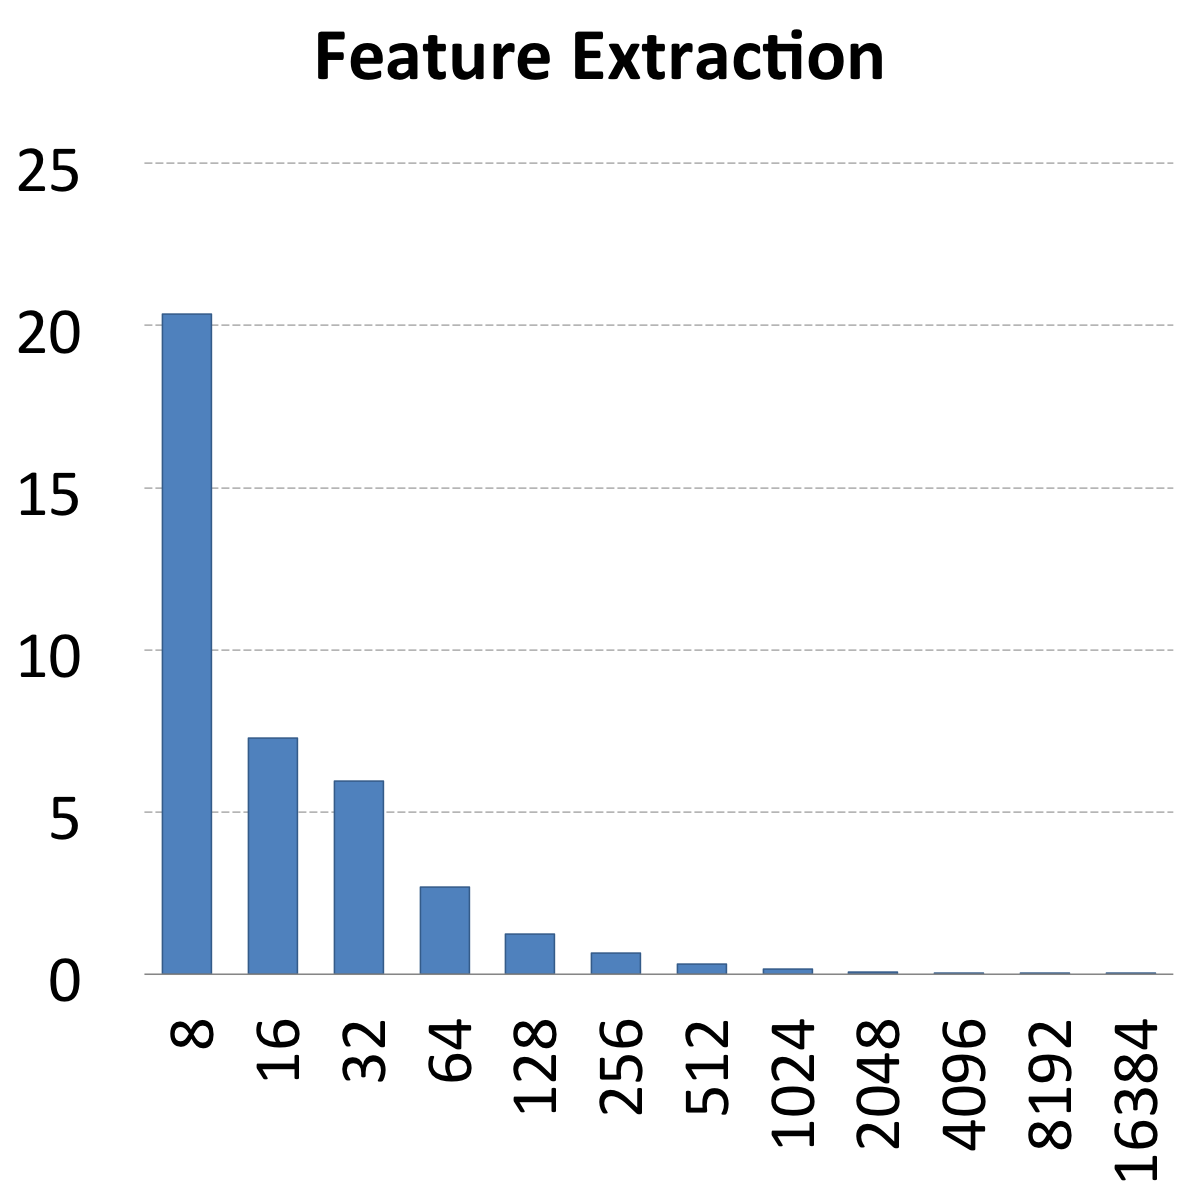
\includegraphics[width=1.0\linewidth]{feature_extraction.png}\\
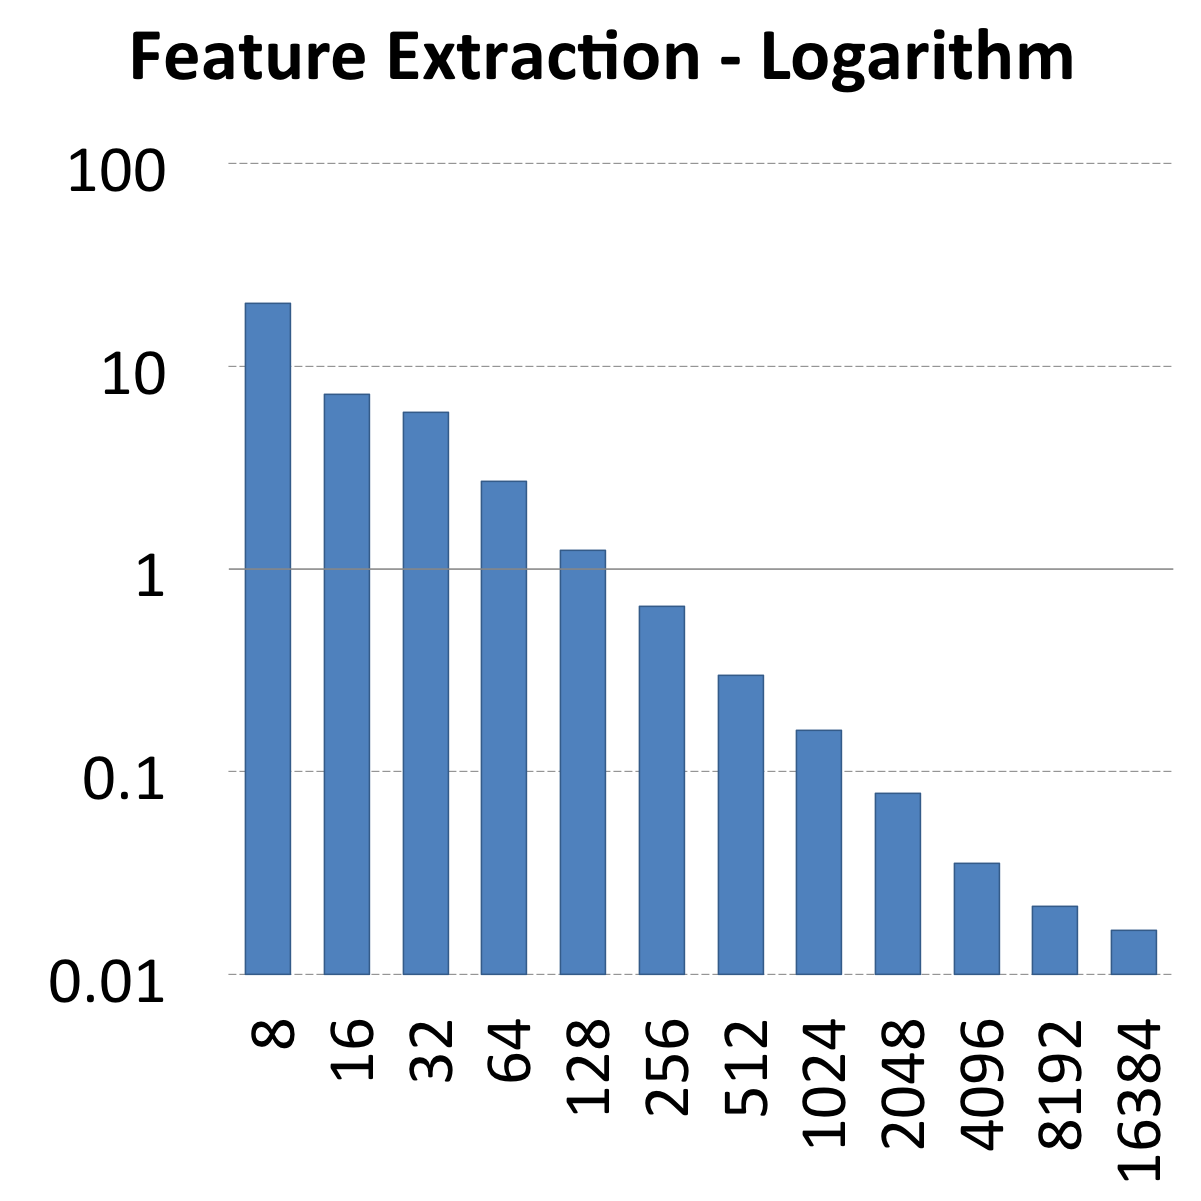
\includegraphics[width=1.0\linewidth]{feature_extraction_log.png}
\caption{Computation time for feature extraction. The top plot is shown in linear scale, and the bottom plot is shown in logarithmic scale. It is linearly scalable as the number of processor increases}
\label{fig:feature-extraction}
\end{figure}

\textbf{Create Local Connectivity Tree ($T_{create}$)}
%
Despite the size of each data block, the computation cost for creating and updating local connectivity tree is dependent on the number of the features extracted within the original volume, or more precisely, the number of features that touches the boundary surface of their residing data block. As shown in Figure~\ref{fig:create-local-graph}, similar to $T_{extract}$, $T_{create}$ decreases as the number of processors increases in post-processing, as the the number of feature-on-boundary decreases accordingly. For the combustion data set, it takes an average of 0.1 seconds to create the local connectivity tree, approximately 0.5\% the time of $T_{extract}$ using the same amount of processors. This portion increases but does not succeed 1\% in out test, hence $T_{create}$ is not considered as a bottleneck. %\textcolor{red}{for in-situ visualization however... }

\begin{figure}[t]
\centering
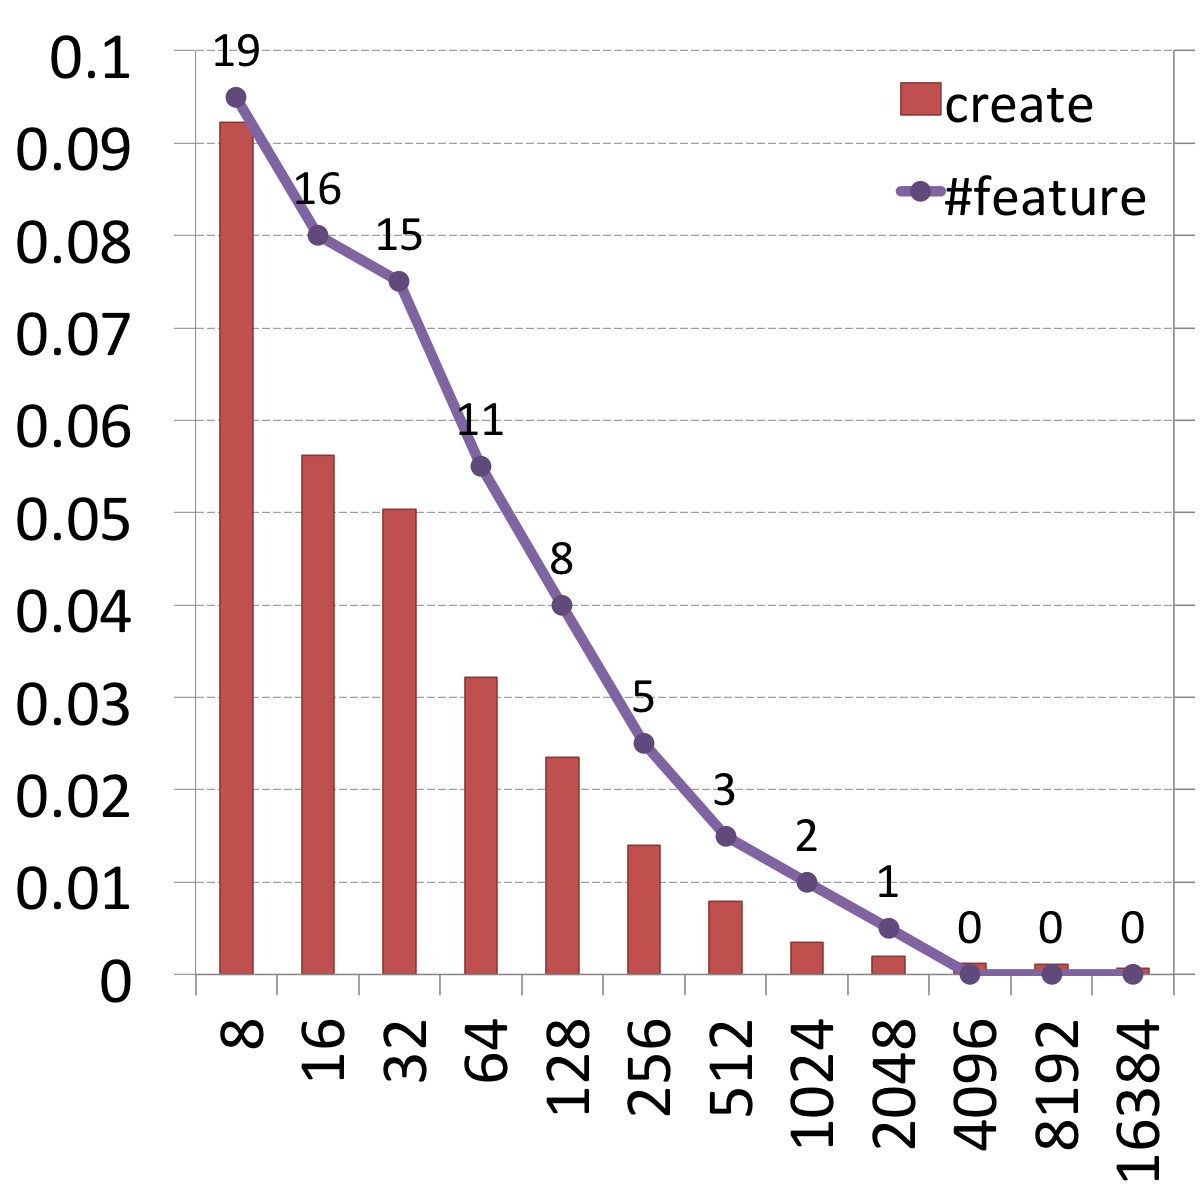
\includegraphics[width=1.0\linewidth]{create_local_graph.png}
%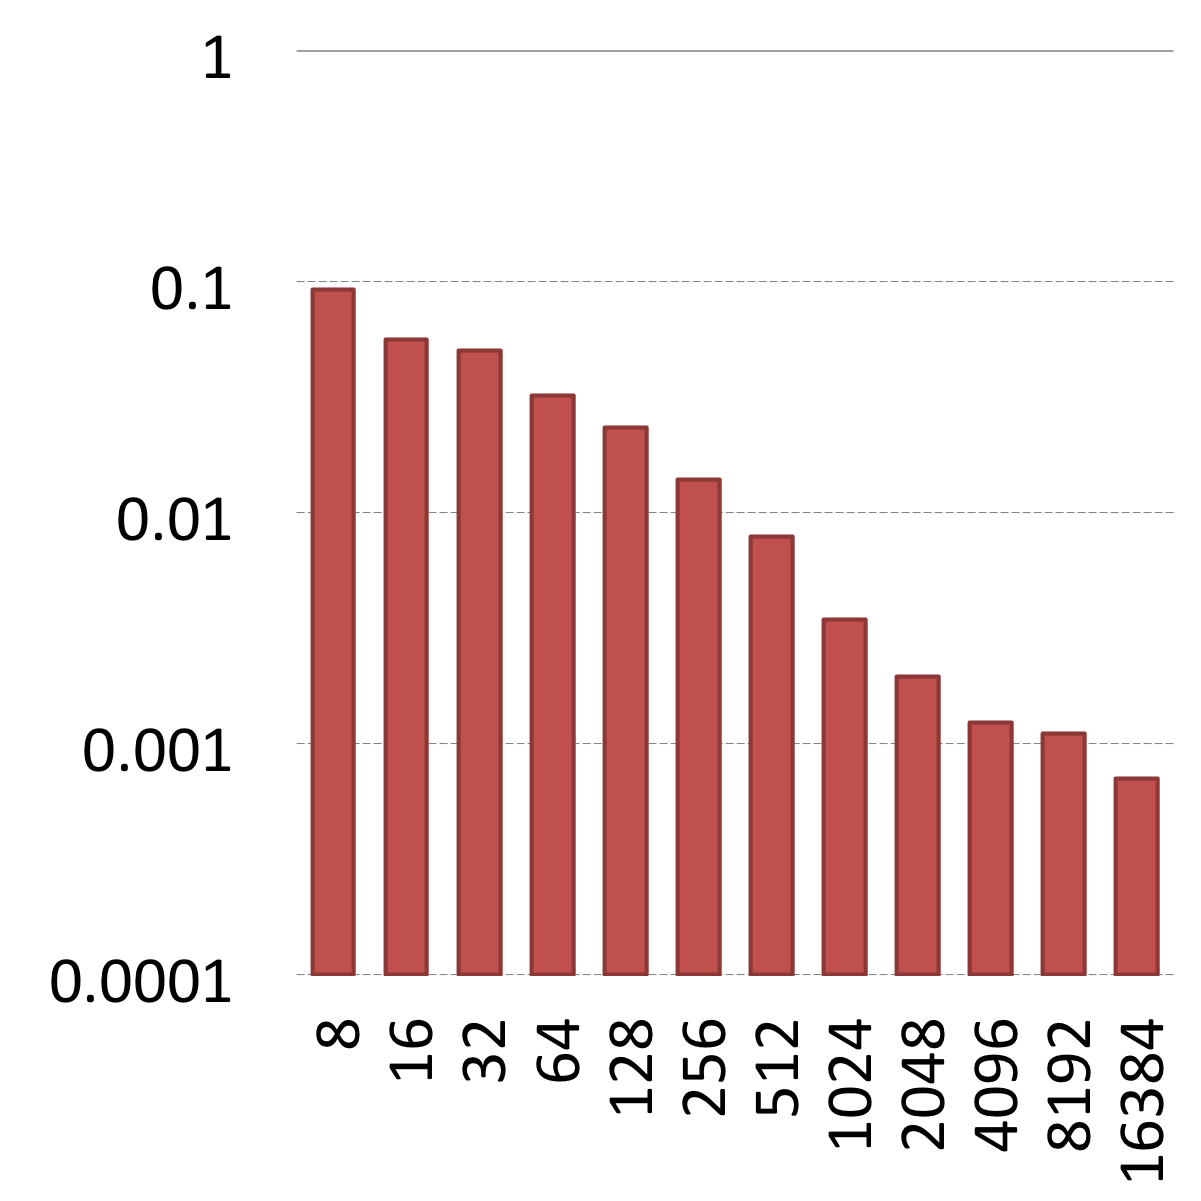
\includegraphics[width=0.6\linewidth]{create_local_graph_log.png}
\caption{Computation time for creating local connectivity tree. It is linearly scalable as the number of processor increases. The time is approximately proportional to the number of features-on-boundary. Note that, for the processor number greater than 4096, the average feature number is between 0 and 0.5 and is rounded to 0.}
\label{fig:create-local-graph}
\end{figure}

\textbf{Create Global Connectivity Information ($T_{merge}$)}
%
We also test the centralized approach and the decentralized approach in creating global connectivity information that is the major factor related to the scalability of our algorithm. Though the number of features-on-boundary decreases as more processors involved, the communication time for the centralized approach increases as $N_p$ increases. According to the comparison depicted in Figure~\ref{fig:local-vs-global}, we can see that the centralized approach is suitable for the scenarios that we only need a small number of processors, and the decentralized approach for creating connectivity information using a relatively large amount of the processors.

\begin{figure}[ht]
\centering
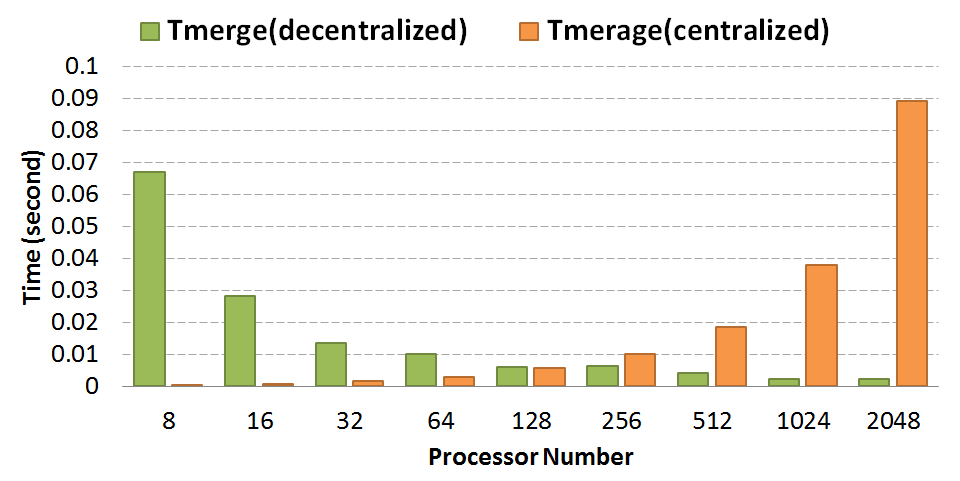
\includegraphics[width=1.0\linewidth]{local_vs_global.png}
\caption{The comparison between the computation time for the centralized approach and the decentralized approach. The centralized approach works well for a small number of processors while the decentralized approach exceeds after a certain number, 128 processors for the combustion data set, is used.}
\label{fig:local-vs-global}
\end{figure}

As shown in Figure~\ref{fig:global-merge}, the total time $T_{merge}$ for the centralized approach exceeds $T_{extract}$ after certain amount of processors, 2048, for the combustion data set, which makes the overall execution time rebounds . On the other hand, the decentralized approach  scales well up to 16384 processors for the combustion data set, as the communication cost is as low as ${O(\sqrt[3]{N_p})}$.

\begin{figure}[t]
\centering
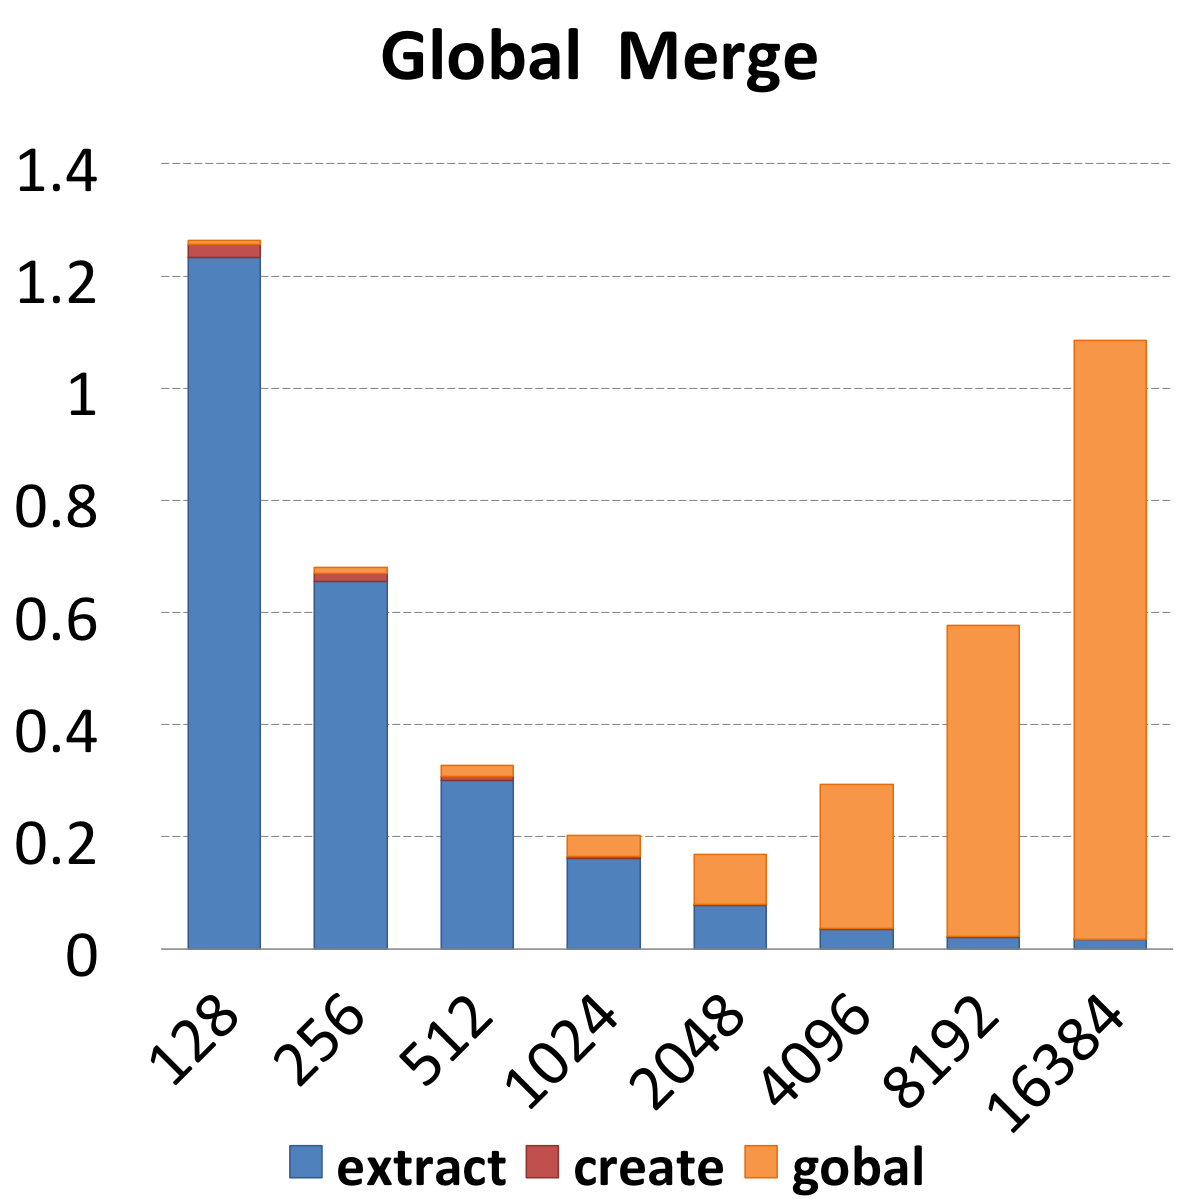
\includegraphics[width=1.0\linewidth]{global_merge.png}\\
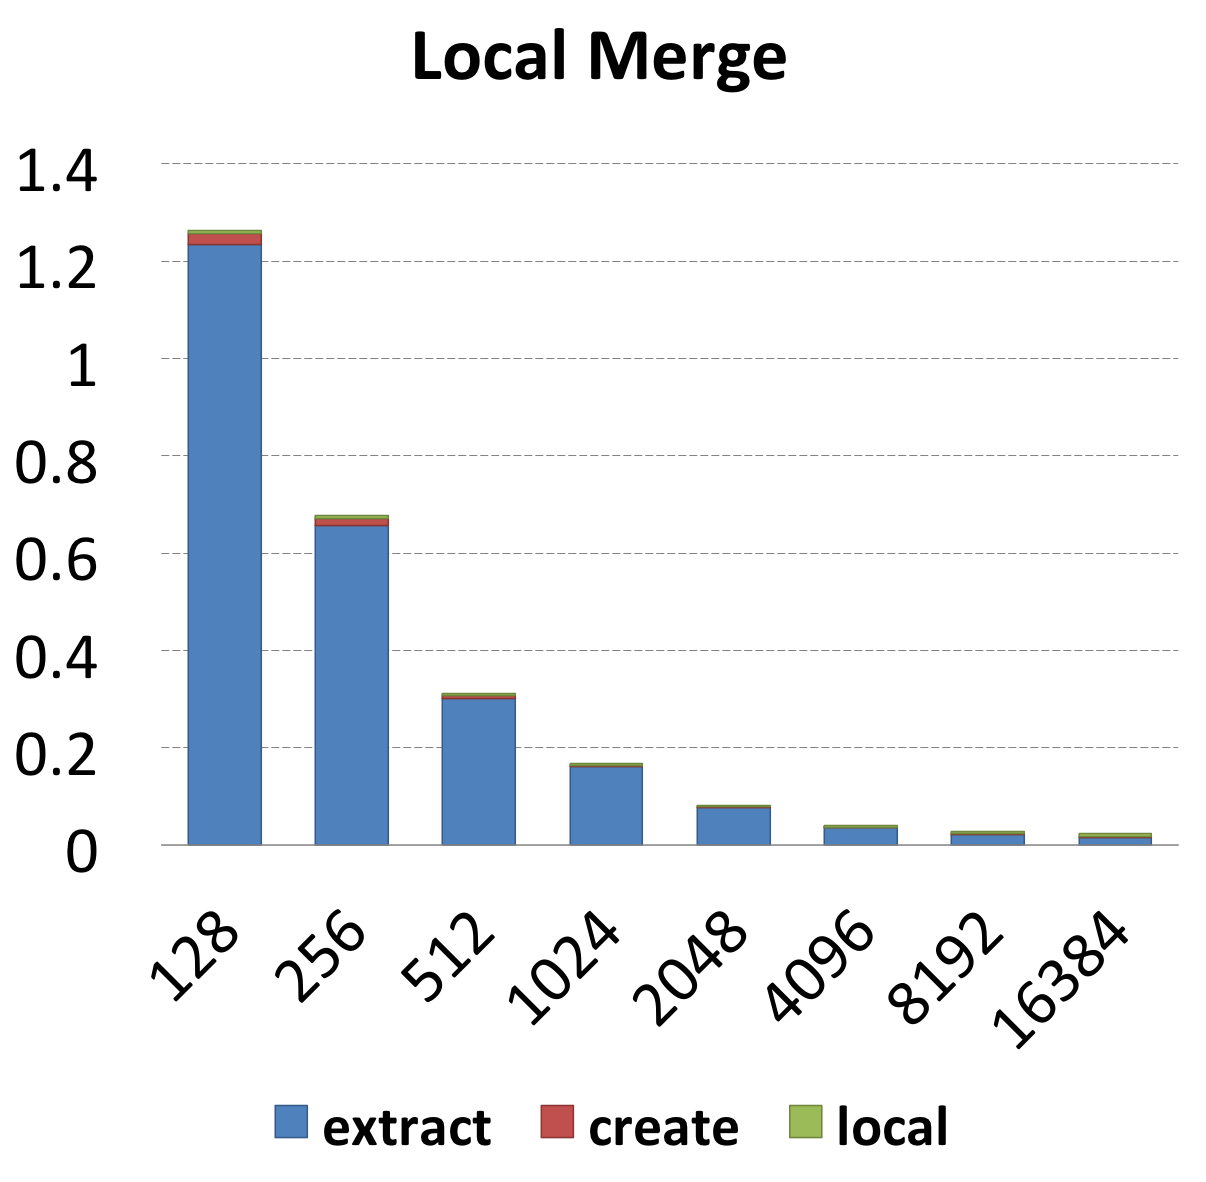
\includegraphics[width=1.0\linewidth]{local_merge.png}
\caption{Total computation time comparison for different merging strategy. The decentralized-global-merge strategy scaled up to 2048 processors but the merging time outweighs the extraction time when using more processors; The decentralized-local-merge strategy scaled log-linearly up 16384 processors for the combustion data set.}
\label{fig:global-merge}
\end{figure}



\section{Conclusion}
\textcolor{red}{To be revised}
In this paper, we presented a decentralized approach that all feature connectivity information are created and preserved among distributed processors. Traditional approaches perform connectivity test on each processor and subsequently correspond them in a host processor after gathering all or partially merged connectivity information. Our approach does not follow this paradigm. Rather, instead being sent back to the host, the local connectivity information are computed and preserved only in the local processor.
There is no copy of the global feature information preserved in the host, and the host only acts as the interface from where the criterion of feature of interest is broadcast. In this way, the computation of merging local connectivity information is distributed to the slaves, which can effectively remove the potential communication bottleneck on the host processor.
Moreover, there's no need to set a barrier and wait for all connectivity information being sent back to the host, thus if one of the features spans over a large number of processors but was not selected by the user, the potentially long computation time for this feature will not be considered. This makes it ideal for an interactive system, where users can select the feature of interest and instantly receive the visual feedback as the feature evolves.


% references section

\bibliographystyle{IEEEtran}
\bibliography{ptrack}

% <OR> manually copy in the resultant .bbl file
% set second argument of \begin to the number of references
% (used to reserve space for the reference number labels box)
%\begin{thebibliography}{1}
%\end{thebibliography}

\end{document} 